\section{Introduction}
\label{sec:intro}

\subsection{Motivation and the failure that defined the question}

Ant scans can turn specimens that are difficult to measure repeatedly into a
source of comparable three-dimensional traits. If every scan is registered to
a common parametric model, quantities such as head width, Weber's length or
appendage proportions can be extracted systematically instead of by hand under
a microscope, which opens a route to studying morphological diversity at
population scale; recent work on \emph{Atta} workers already shows that a 3D
shape space can reveal structure that size scaling alone does not~\cite{imirzian}.
Real scans, however, whether from scAnt photogrammetry~\cite{scant} or
micro-CT, are far from ideal inputs: they contain holes, self-intersections,
arbitrary orientation and missing surface exactly at the thin structures of
greatest anatomical interest (Figure~\ref{fig:raw-scans}).

\begin{figure}[!htb]
\centering
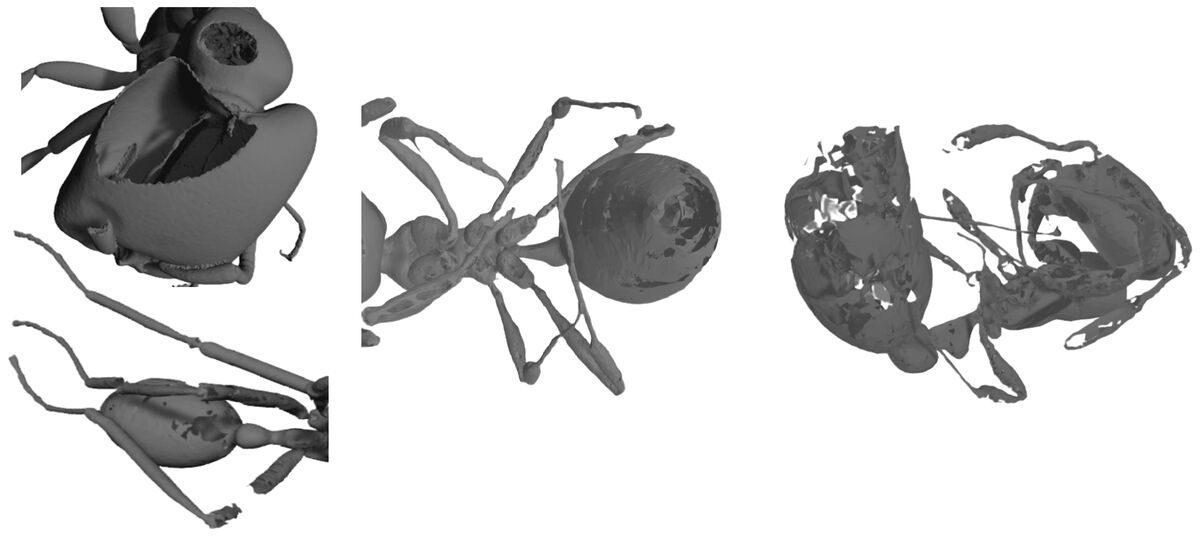
\includegraphics[width=0.6\linewidth]{figures/fig_before_registration.jpg}
\caption[Raw scans before registration]{Raw scans before registration: holes,
self-intersections and missing surface at the structures of greatest
anatomical interest.}
\label{fig:raw-scans}
\end{figure}

The method studied here, SMILify, builds on SMALify~\cite{smalify}, an
optimisation-based framework for fitting the SMAL quadruped model~\cite{smal}.
Its ambition is to turn any rigged mesh into a SMAL-compatible parametric
model, with SMIL (Skinned Multi-Insect Linear) as the current insect-focused
instance. At the outset, of roughly 380 raw scans in the available corpus only
86 (about 23\%) had been curated as clean enough for registration.

In the first week of July 2026, ten preprocessed ant scans were passed through
the registration pipeline. All ten optimisations converged cleanly: the loss
curves showed no divergence and the objective decreased as expected. Four of
the resulting models were nevertheless not recognisable as anatomically
meaningful ants. Legs had collapsed into the gaster and, in some fits, the head
had been absorbed into the thorax. More troublingly, several of these wrong
fits reached a \emph{lower} loss than the runs that had visibly succeeded. The
optimiser had succeeded; the registration had failed. This discrepancy is the
starting point of the work. The objective is a symmetric point-to-point
distance between two surfaces: it measures whether the fitted mesh
\emph{covers} the target, not whether vertex $i$ of the template has landed on
the anatomical point it is defined to represent. When the two diverge, nothing
in the pipeline's own numerical output signals it.

\subsection{The problem: recovering a latent explanation}
\label{sec:problem}

Registration recovers, for a scan $T$, the latent variables of a parametric
mesh $M$: shape $\bm\beta$, articulated pose $\bm\theta$, scale $s$ and
residual per-vertex deformation $\mathbf d$,
\begin{equation}
(\hat{\bm\beta},\hat{\bm\theta},\hat s,\hat{\mathbf d})
 =\arg\min_{\bm\beta,\bm\theta,s,\mathbf d}\;
 \mathcal{L}\big(M(\bm\beta,\bm\theta,s,\mathbf d),\,T\big).
\label{eq:registration}
\end{equation}
The scan is only a set of surface samples. It carries no vertex identities, no
joint locations and no anatomical labels, yet these are exactly the quantities
the registration is meant to deliver. Anatomical correspondence is therefore an
intended \emph{consequence} of the recovered parameters, not something the
objective observes. Because Equation~\eqref{eq:registration} is non-convex and
its objective sees surfaces only, several different latent configurations can
generate nearly the same surface: the mapping from observed surface to
anatomical state is not guaranteed to be identifiable.

This is the idea around which the report is organised. The hard part is not
optimising a mesh to a scan; it is recovering the \emph{correct} articulated
explanation from an observation that does not contain anatomical identity. Each
investigation below is a different way of interrogating that one problem
(Figure~\ref{fig:map}): asking whether the observation is good enough, whether
the search can reach the right explanation, what extra information would
disambiguate it, how much freedom lets a wrong explanation hide, and finally
whether an independent reference confirms the result. Four research questions
make this precise:
\begin{enumerate}[label=\textbf{RQ\arabic*.}]
\item Is input mesh quality the dominant limit on registration accuracy?
\item Does a good surface fit imply a correct anatomical fit?
\item Which component (initialisation, sampling, deformation freedom,
correspondence or the objective) limits anatomical recovery, and where along
the body?
\item When a parameter is recovered, when is it a valid biological
measurement?
\end{enumerate}

\begin{figure}[!htb]
\centering
\begin{tikzpicture}[every node/.style={font=\small},
 n/.style={draw,rounded corners=2pt,minimum height=8mm,align=center,fill=white,inner sep=3pt},
 q/.style={font=\footnotesize\itshape,align=center,text width=3.4cm},
 arr/.style={-{Stealth[length=2mm]}}]
\node[n,fill=gray!12] (o) {Observation\\scan surface $T$};
\node[n,right=2.6cm of o] (l) {Latent explanation\\$\bm\beta,\bm\theta,s,\mathbf d$};
\node[n,right=2.6cm of l,fill=blue!10] (a) {Anatomical identity\\(never observed)};
\draw[arr](o)--(l); \draw[arr](l)--(a);
\node[q,below=4mm of o] {Is the observation good enough? (RQ1)\\preprocessing};
\node[q,below=4mm of l] {Can the search reach the right explanation? Is it unique? (RQ3)\\initialisation, sampling, robust optimisation, deformation freedom};
\node[q,below=4mm of a] {What would disambiguate it, and can it be verified? (RQ2, RQ4)\\anatomical priors, correspondence, joint supervision, expert truth};
\end{tikzpicture}
\caption[One inverse problem, several investigations]{The report treats
registration as one inverse problem. Each investigation interrogates a
different link between the observed surface, the recovered parameters and the
anatomical identity that was never observed.}
\label{fig:map}
\end{figure}

\subsection{Objectives and contribution}

The internship brief listed six assignments: unify the preprocessing pipeline,
stabilise a Shape-Diameter-Function-based segmentation, integrate neural
initialisation, design a hybrid registration framework, benchmark the result
and deliver documentation. Read together they imply a hypothesis, that input
mesh quality is the limiting factor. A controlled test of that hypothesis was
negative (\F{F2}), and the work was redirected, with my supervisor, toward the
questions above.

SMILify already provided the parametric representation and a baseline fitting
pipeline. The contribution of this work is the diagnostic and validation
machinery built around it and what that machinery established. It is a
framework for making articulated 3D reconstruction \emph{measurable,
diagnostically interpretable and independently verifiable}: a synthetic
round-trip benchmark with exact vertex identity, counterfactual (oracle)
interventions, a three-level evaluation protocol, a corrected and frozen expert
benchmark, and several algorithmic and systems extensions, each judged against
a criterion fixed before the experiment (Table~\ref{tab:contrib}). The central
result is that surface agreement, anatomical correspondence, parameter
recovery and measurement validity are related but distinct properties that do
not track one another.

\subsection{Structure of the report}

Section~\ref{sec:host} presents the host organisation: its domain of activity,
its structure and the professions present. Section~\ref{sec:work} describes and
analyses the work and its place in the institute, following the argument above:
the problem and the experimental design, then the investigations of
observation, objective, information and measurement validity.
Section~\ref{sec:conclusion} concludes with limitations, outlook and what the
internship taught me.
